
\documentclass[conference,compsoc]{IEEEtran}

\ifCLASSOPTIONcompsoc

  \usepackage[nocompress]{cite}
\else

  \usepackage{cite}

\fi

\ifCLASSINFOpdf
   \usepackage[pdftex]{graphicx}
\else
  
\fi


\hyphenation{op-tical net-works semi-conduc-tor}
\usepackage{float}
\usepackage{hyperref}
\usepackage{xcolor}

\begin{document}

\title{Privacy Preserving Decision Tree Prediction}

\author{\IEEEauthorblockN{Reem Younis, Assia Khateeb, Atheer Abo Foul, Aya Miari\IEEEauthorrefmark{0}
\IEEEauthorblockA{\IEEEauthorrefmark{0}Lecturer : Dr. Adi Akavia, Laboratory in Privacy Preserving Machine Learning, 
University of Haifa\\
Email: reembyounis@gmail.com, assia.khteb@gmail.com, 19aether6@gmail.com, aia-m-211@hotmail.com\IEEEauthorrefmark{0}}
}
}

% make the title area
\maketitle
\textbf{\large{Part A:}}
\tableofcontents

\newpage
\begin{abstract}
In machine learning, the decision tree is an algorithm for supervised learning for classification. The algorithm allows for learning, in that it processes elements in the training set one at a time.We implement decision tree algorithm on clear-text dataset. Then, we test accuracy of our decision tree algorithm classification results. \\

\end{abstract}


\section{Introduction}

Reference to our \href{https://github.com/assiakhateeb/PPML_lab/tree/main/Part\%20A}{\textcolor{blue}{Github repo}}.\\
Decision Tree algorithm belongs to the family of supervised learning algorithms. Unlike other supervised learning algorithms, decision tree algorithm can be used for solving regression and classification problems too.

The general motive of using Decision Tree is to practice it .\\
Decision Tree represents a procedure for classifying data based on attributes or features. It is also an efficient way of processing data ,for this very reason it has wide application in data mining.\\
In Decision Tree structure each internal node represents a "test" on an attribute, each branch represents the outcome of the test, and each leaf node represents a class label. The paths from root to leaf represent classification rules.\\
This data structure is quite intuitive and easy to assimilate by humans.




\section{Methodology}


The working model of decision tree is quite easy to implement and can be very effective in most of the classification problems. \\
In our decision tree, for predicting a class label for a dataset We compare the values of the root attribute with dataset’s attribute. On the basis of comparison, we follow the branch corresponding to that value and jump to the next node.

We continue comparing our dataset’s attribute values with other internal nodes of the tree until we reach a leaf node with predicted class value.
\subsection{Prediction And Samples}
Assumptions we make while using Decision Tree :
\\ \textit{1.} At the beginning, we consider the whole training set as the root.
\\ \textit{2.} Attributes are assumed to be categorical for information gain and for gini index, attributes are assumed to be continuous.
\\ \textit{3.} On the basis of attribute values records are distributed recursively.
\\ \textit{4.} We use statistical methods for ordering attributes as root or internal node.

\subsection{Attribute Selection Measures}

Attribute selection measure is a heuristic for selecting the splitting criterion that partition data into the best possible manner. It is also known as splitting rules because it helps us to determine breakpoints for tuples on a given node. ASM provides a rank to each feature(or attribute) by explaining the given data set. Best score attribute will be selected as a splitting attribute (Source). In the case of a continuous-valued attribute, split points for branches also need to define. Most popular selection measures are Information Gain, Gain Ratio, and Gini Index.

\subsection{Entropy}

In physics and mathematics, entropy referred as the randomness or the impurity in the system. In information theory, it characterizes the impurity of an arbitrary collection of examples.
Entropy is the measure of uncertainty of a random variable, The higher the entropy the more the information content.
\\ The entropy can explicitly be written as:
\\ H(X) = $\sum_{n=1}^{N}p(x_i)\log_{2}p(x_i)$

   
By calculating entropy measure of each attribute we can calculate their information gain. Information Gain calculates the expected reduction in entropy due to sorting on the attribute. Information gain can be calculated. 

\subsection{Information Gain}

Information gain is the decrease in entropy. Information gain computes the difference between entropy before split and average entropy after split of the data set based on given attribute values.
\\ Definition: Suppose S is a set of instances, A is an attribute, $\S_v$ is the subset of S with A=v and Values(A) is the set of all possible of A, then \\ Gain(S,A) = Entropy(S) - $\sum_{v:val(A)} |S_v| Entropy(|S_v|)$
\\ $|S|$ denotes the size of set S


\subsection{Gini index}

Another decision tree algorithm CART (Classification and Regression Tree) uses the Gini method to create split points.
\\ Gini index and Information Gain both of these methods are used to select from the n attributes of the dataset which attribute would be placed at the root node or the internal node.
\\ Gini index = 1 - $\sum_{j} P_j^2$


\section{Algorithm }
How the algorithm works?\\
\textit{1.} Select the best attribute using Attribute Selection Measures(ASM) to split the records.
\\\textit{2.} Make that attribute a decision node and breaks the dataset into smaller subsets.
\\\textit{3.} Starts tree building by repeating this process recursively for each child until one of the condition will match:
\\ \textendash All the tuples belong to the same attribute value.
\\\textendash There are no more remaining attributes.


\subsection{Pruning Strategy}
To prune each node one by one (except the root and the leaf nodes), and check weather pruning helps in increasing the accuracy, if the accuracy is increased, prune the node which gives the maximum accuracy at the end to construct the final tree (if the accuracy of 100\% is achieved by pruning a node, stop the algorithm right there and do not check for further new nodes).

\section{Decision Tree - Python}
\subsection{driver.py}
This file gets input from online sources (for example IRIS data "https://archive.ics.uci.edu/ml/machine-learning-databases/iris/iris.data"). 
\\ In addition, all the functions in DecisionTree.py are called in this file. For example : build$\_$tree, getLeafNodes, getInnerNodes, computreAccuracy, print$\_$tree.


\subsection{DecisionTree.py}
\underline{function build$\_$tree} : a recursice function that returns the final tree.
\\rows - contains number of objects.
\\header - contains number of columns/features/labels.
\\\underline{function find$\_$best$\_$split} : returns best question that could be asked so far, in addition to best information gain.
\\rows,header refer to the same as in build$\_$tree.
\\\underline{function Leaf} : initializes the leaf data.
\\\underline{function partition} : checks if a question matches an object, if yes then add to true$\_$rows, if no add to false$\_$rows.
\\ returns two arrays, true$\_$rows,false$\_$rows.
\\\underline{function Decision$\_$Node} : This holds a reference to the question, and to the two child nodes.






\section{Datasets }
\large{\textbf{Drug}}\\
The dataset contains various information that effect the predictions like Age, Sex, BP, Cholesterol levels, Na to Potassium Ratio and finally the drug type. \\

\underline{The target feature is:}
\\ \textendash Drug type\\

\underline{The feature sets are:}\\
   \textit{1.} Age\\
   \textit{2.} Sex\\
    \textit{3.}Blood Pressure Levels (BP)\\
   \textit{4.} Cholesterol Levels\\
   \textit{5.} Na to Potassium Ration\\
   
\begin{figure}[H]
\centering
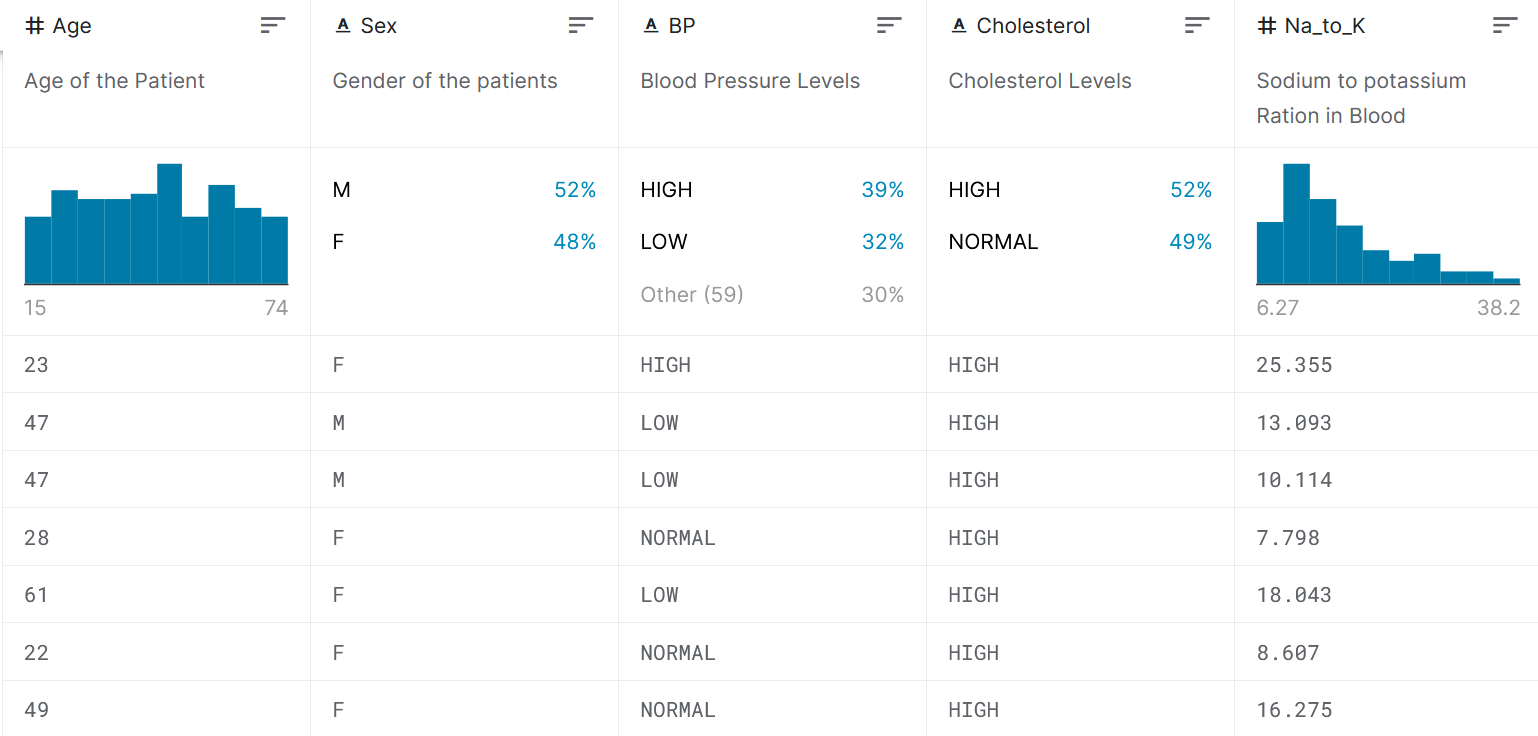
\includegraphics[width=6in,height=2.8in]{drug dataset.PNG}

\caption{Drug Classification Dataset }
\label{fig_error}

\end{figure}  


\section{Results}

 \subsection{Sample outputs (Drug Classification Dataset)}
 \textendash Accuracy before pruning: 97.0\%
\\\textendash Accuracy after pruning: 97.0\%
 \\Pruning strategy did not increased accuracy
 \\\textendash Final Tree with accuracy: 97.0\%
 


 
 

\end{document}
